\documentclass[11pt, a4paper, openany]{book}%twoside

%---------------- Geometry ----------------%
\usepackage[
  a4paper,
  margin=2.0cm, % 1.5cm
  tmargin=2.5cm,
  bmargin=2.5cm,
  %bindingoffset=1cm
]{geometry}

%---------------- Fonts ----------------%
\usepackage[T1]{fontenc}
\usepackage{lmodern}
\linespread{1.2}


%---------------- Math ----------------%
% Use default Computer Modern math fonts
\usepackage{amsmath}
\usepackage{amsfonts}
% \usepackage{amssymb}
\usepackage{braket}

\numberwithin{equation}{chapter}

\DeclareMathOperator{\tr}{tr}

%---------------- Colors ----------------%
\usepackage[table,dvipsnames]{xcolor}
\definecolor{linkblue}{rgb}{0.020, 0.000, 0.478}
\definecolor{linkred}{rgb}{0.459, 0.078, 0.047}
\definecolor{tocgray}{rgb}{0.3, 0.3, 0.3} 
\definecolor{sectiongray}{rgb}{0.2, 0.2, 0.2}
\definecolor{darkgreen}{rgb}{0.0, 0.39, 0.0}
\definecolor{vibrantred}{rgb}{0.86, 0.07, 0.24}

%---------------- Sections ----------------%
\usepackage{sectsty}
\chapterfont{\Huge\color{sectiongray}} 
\sectionfont{\Large\color{sectiongray}} 
\subsectionfont{\large\color{sectiongray}}

%---------------- Tables ----------------%
\usepackage{array}
\usepackage{tabularx}
\usepackage{multirow}
\usepackage{multicol}
\usepackage{booktabs}

%---------------- Graphics ----------------%
\usepackage{graphicx}
\graphicspath{{images}}
\usepackage{wrapfig}
\usepackage{subcaption}
\usepackage{afterpage}
\usepackage[format=hang, labelfont=sc, font=small]{caption} % originally was labelfont=sc

%---------------- Page Layout ----------------%
\usepackage{indentfirst}
\usepackage[page, toc]{appendix}
\usepackage{fancyhdr}
\pagestyle{fancy}
\fancyhead[LE]{\small{\textsc{\leftmark}}}
\fancyhead[LO]{\textsc{\thepage}}
\fancyhead[RE]{\textsc{\thepage}}
\fancyhead[RO]{ \small{\textsc{\rightmark}}}
\cfoot{}
%\renewcommand{\footrulewidth}{0.5pt}
\renewcommand{\headrulewidth}{0.5pt}
\setlength{\headheight}{13.6pt} % Increase header height
\addtolength{\topmargin}{-1.6pt} % Adjust top margin to compensate

%---------------- Theorems ----------------%
\usepackage{amsthm}
\newtheorem*{theorem}{Theorem}
\newtheorem*{lemma}{Lemma}
\newtheorem*{corollary}{Corollary}
\newtheorem*{definition}{Definition}
\newtheorem*{postulate}{Postulate}

%---------------- Custom Commands ----------------%
\newcommand{\question}[1]{\textbf{\textit{\color{vibrantred}[Question: #1]}}}
\newcommand{\comment}[1]{\textbf{\textit{\color{darkgreen}[Comment: #1]}}}

\renewcommand{\thefootnote}{\Roman{footnote}}
\usepackage{perpage} 
\MakePerPage{footnote}

\newcommand{\cst}{\textsf{\textsc{cst}}\xspace}
\newcommand{\qft}{\textsf{\textsc{qft}}\xspace}
\newcommand{\gr}{\textsf{\textsc{gr}}\xspace}
\newcommand{\ctc}{\textsf{\textsc{ctc}}\xspace}

%---------------- Bibliography ----------------%
\usepackage[sorting = none, style=authoryear]{biblatex}
\addbibresource{reflist.bib}

%---------------- Hyperlinks ----------------%
\usepackage{hyperref}
\hypersetup{
    colorlinks=true,
    linkcolor=tocgray,
    citecolor=linkblue,
    urlcolor=darkgreen,
}
\usepackage{cleveref}

%---------------- Misc ----------------%
\usepackage{csquotes}
\usepackage{makeidx}
\makeindex
\usepackage{siunitx}
\usepackage{blindtext}
\usepackage{footmisc}
%\setcounter{tocdepth}{1}

%---------------- Plots ----------------%
\usepackage{tikz}
\usetikzlibrary{patterns}
% \usepackage{pgfplots}

\graphicspath{{figures/}}




\title{Master's thesis}
\author{Jonas Broe Bendtsen}
\date{June 2026}

\begin{document}
\maketitle
\tableofcontents
\chapter{Simsilun}
\section{Comparing LTB to silent universe and simsilun}\label{sec:LTBvsSimsilun}
To test the silent universe and simplified silent universe approximations, I compare the results to the analytical LTB solution.
First, a set of initial conditions is generated from the LTB model. These are the density:
\begin{equation}
    \rho = \frac{2M'}{R^2 R'},
\end{equation}
the expansion:
\begin{equation}
    \Theta = \frac{\dot{R}'}{R'} + 2\frac{\dot{R}}{R},
\end{equation}
the shear:
\begin{equation}
    \Sigma = \frac{1}{3}\left(\frac{\dot{R}}{R} - \frac{\dot{R}'}{R'}\right),
\end{equation}
and the electric part of the Weyl tensor:\question{Is it actually the electric part of the Weyl tensor?}
\begin{equation}
    \mathcal{W} = \frac{M}{R^3}-\frac{M'}{3R^2R'}.
\end{equation}
The volume of each point is calculated by taking the determinant of the spatial part of the metric. Lastly, the backreaction is calculated by integrating (i.e. taking the cumulative sum) from the centre outwards to obtain average values of the expansion $\langle \Theta \rangle_\mathcal{D}$ and its square $\langle \Theta^2 \rangle_\mathcal{D}$, as well as the average shear squared $\langle \Sigma^2 \rangle_\mathcal{D}$. The backreaction is then calculated using \cref{eq:backreaction}. All these quatitites are calculated at an initial redshift of $z=1100$.

The initial conditions are evolved using the simsilun program and compared to the analytical LTB solution at $t_0$. First, all initial conditions are used, hence the simulation just uses the silent universe approximation. After that, only the initial density and volume are used, and the simplified silent universe approximation is used to calculate the remaining initial conditions. The results are shown in \Cref{fig:density,fig:expansion,fig:shear,fig:volume,fig:backreaction}.

\begin{figure}
    \centering
    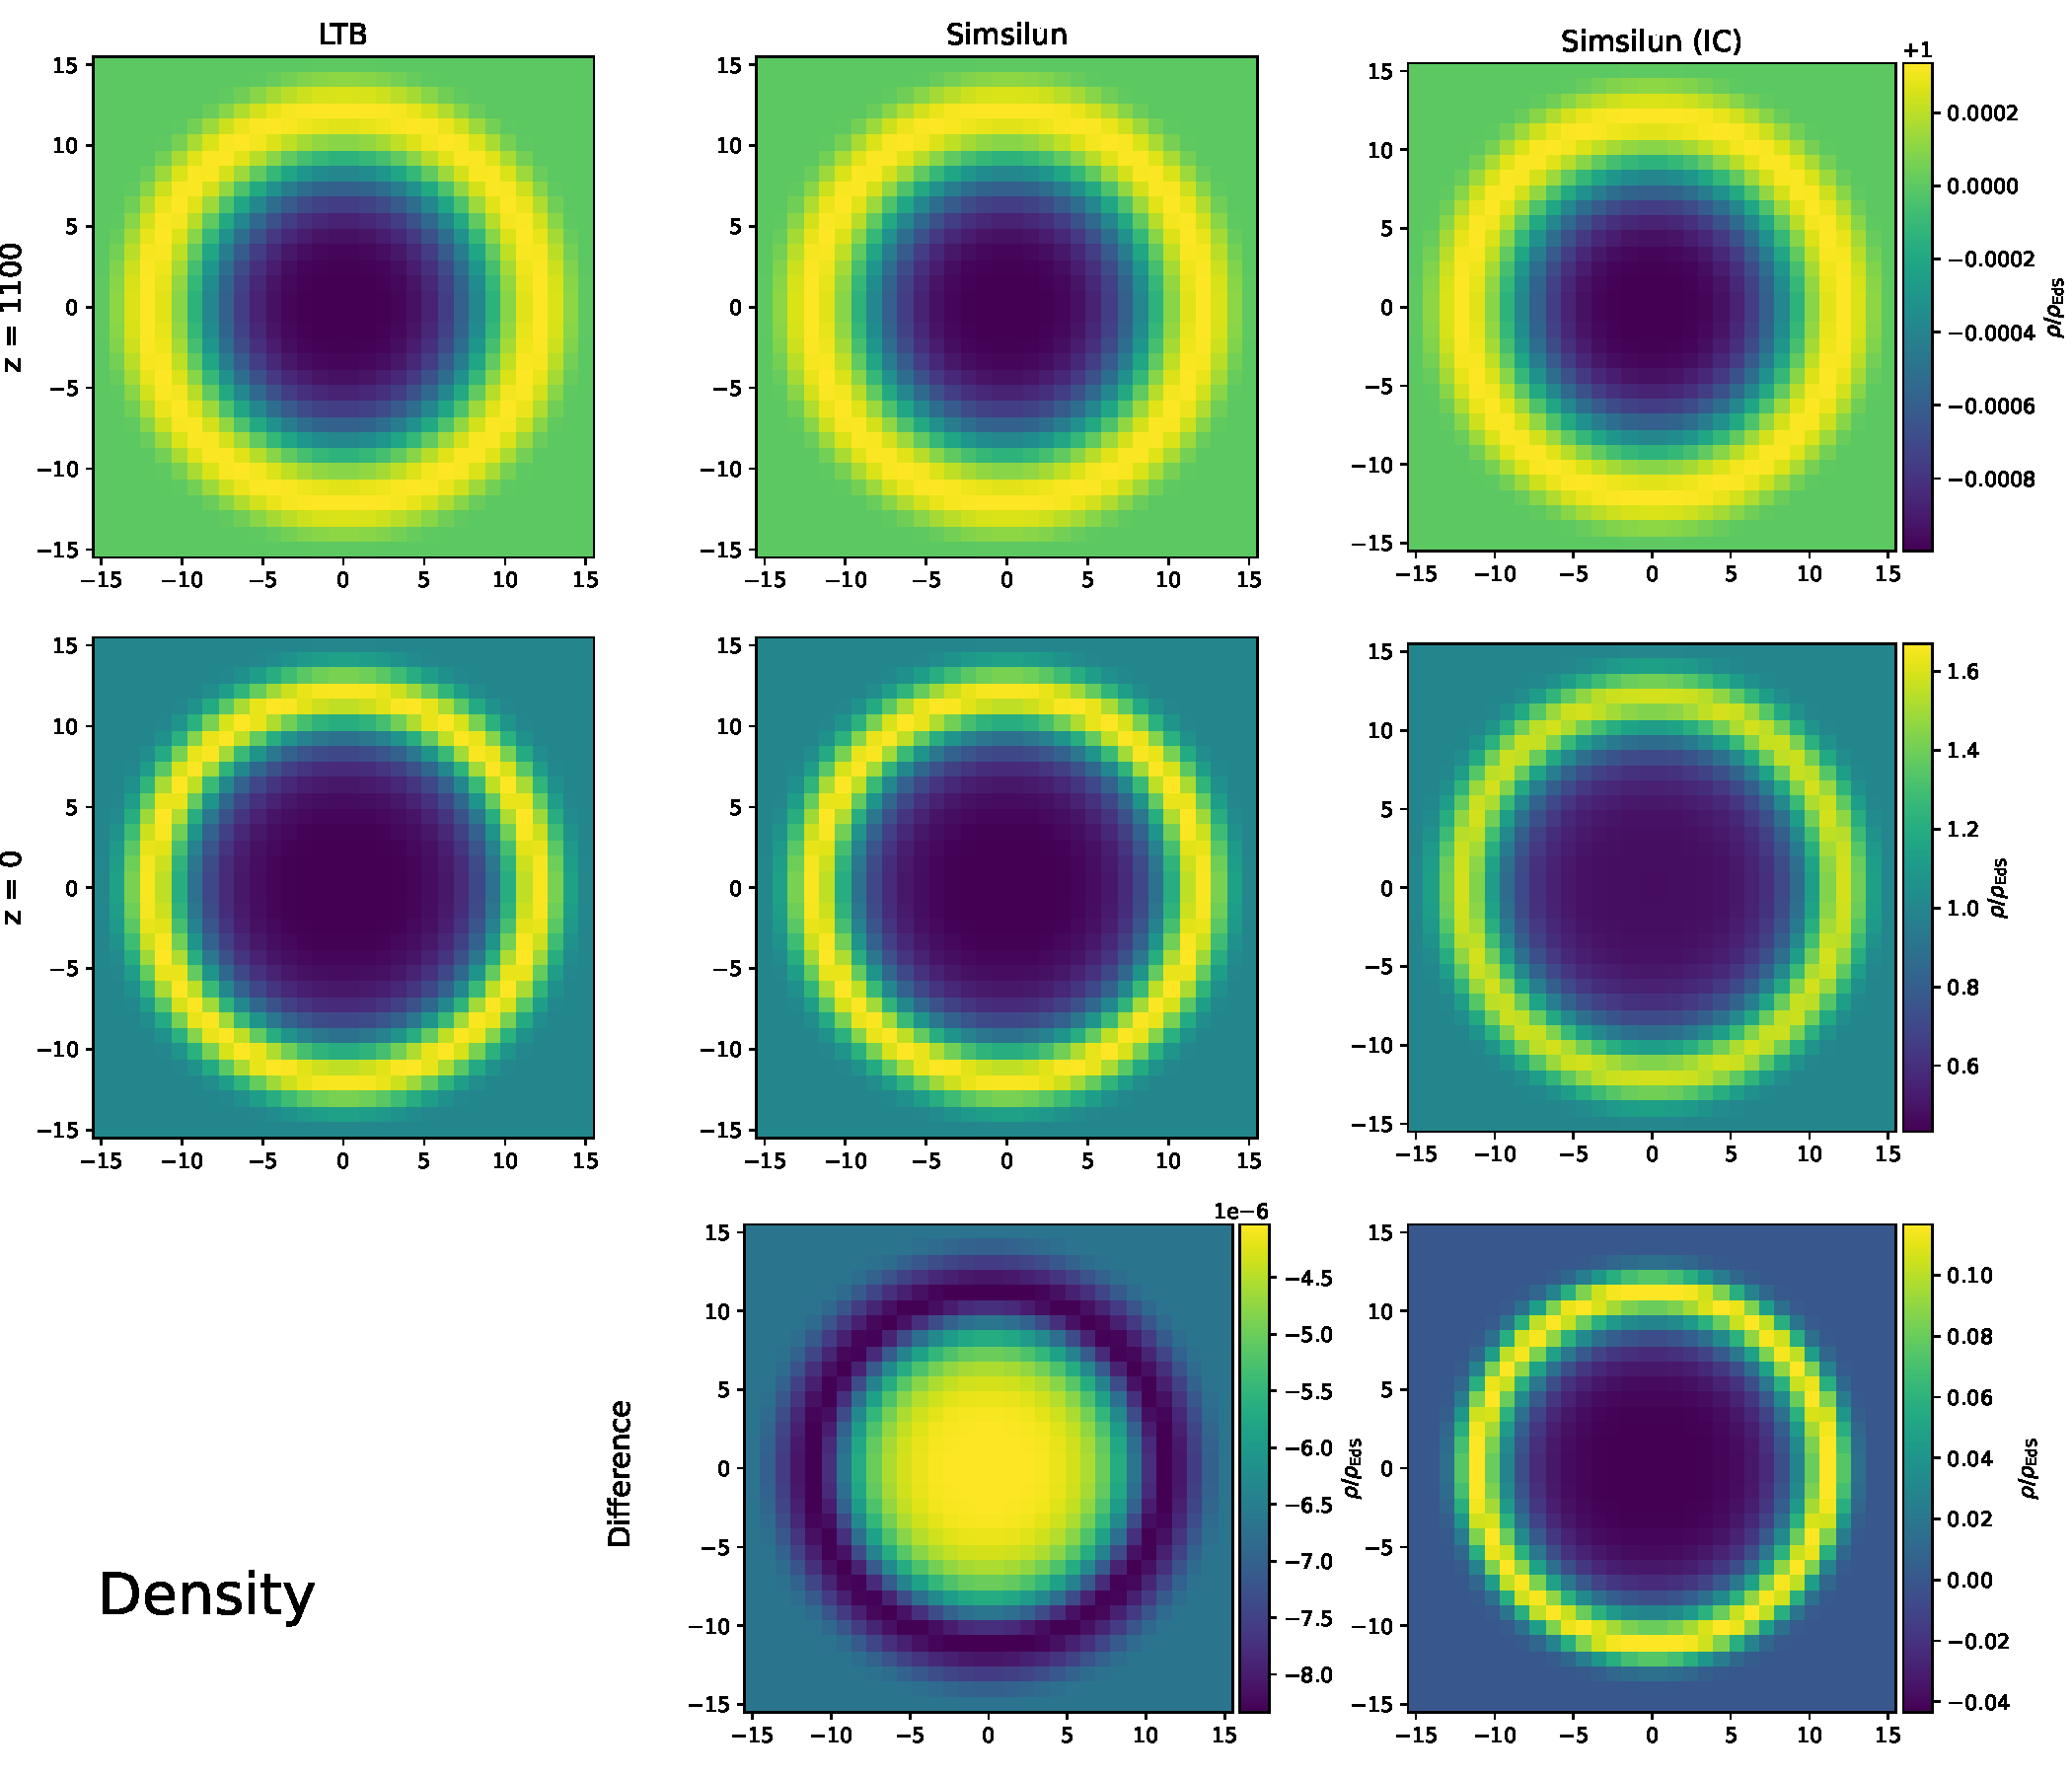
\includegraphics[width=\textwidth]{../plots/Density.pdf}
    \caption{Density}
    \label{fig:density}
\end{figure}



\begin{figure}
    \centering
    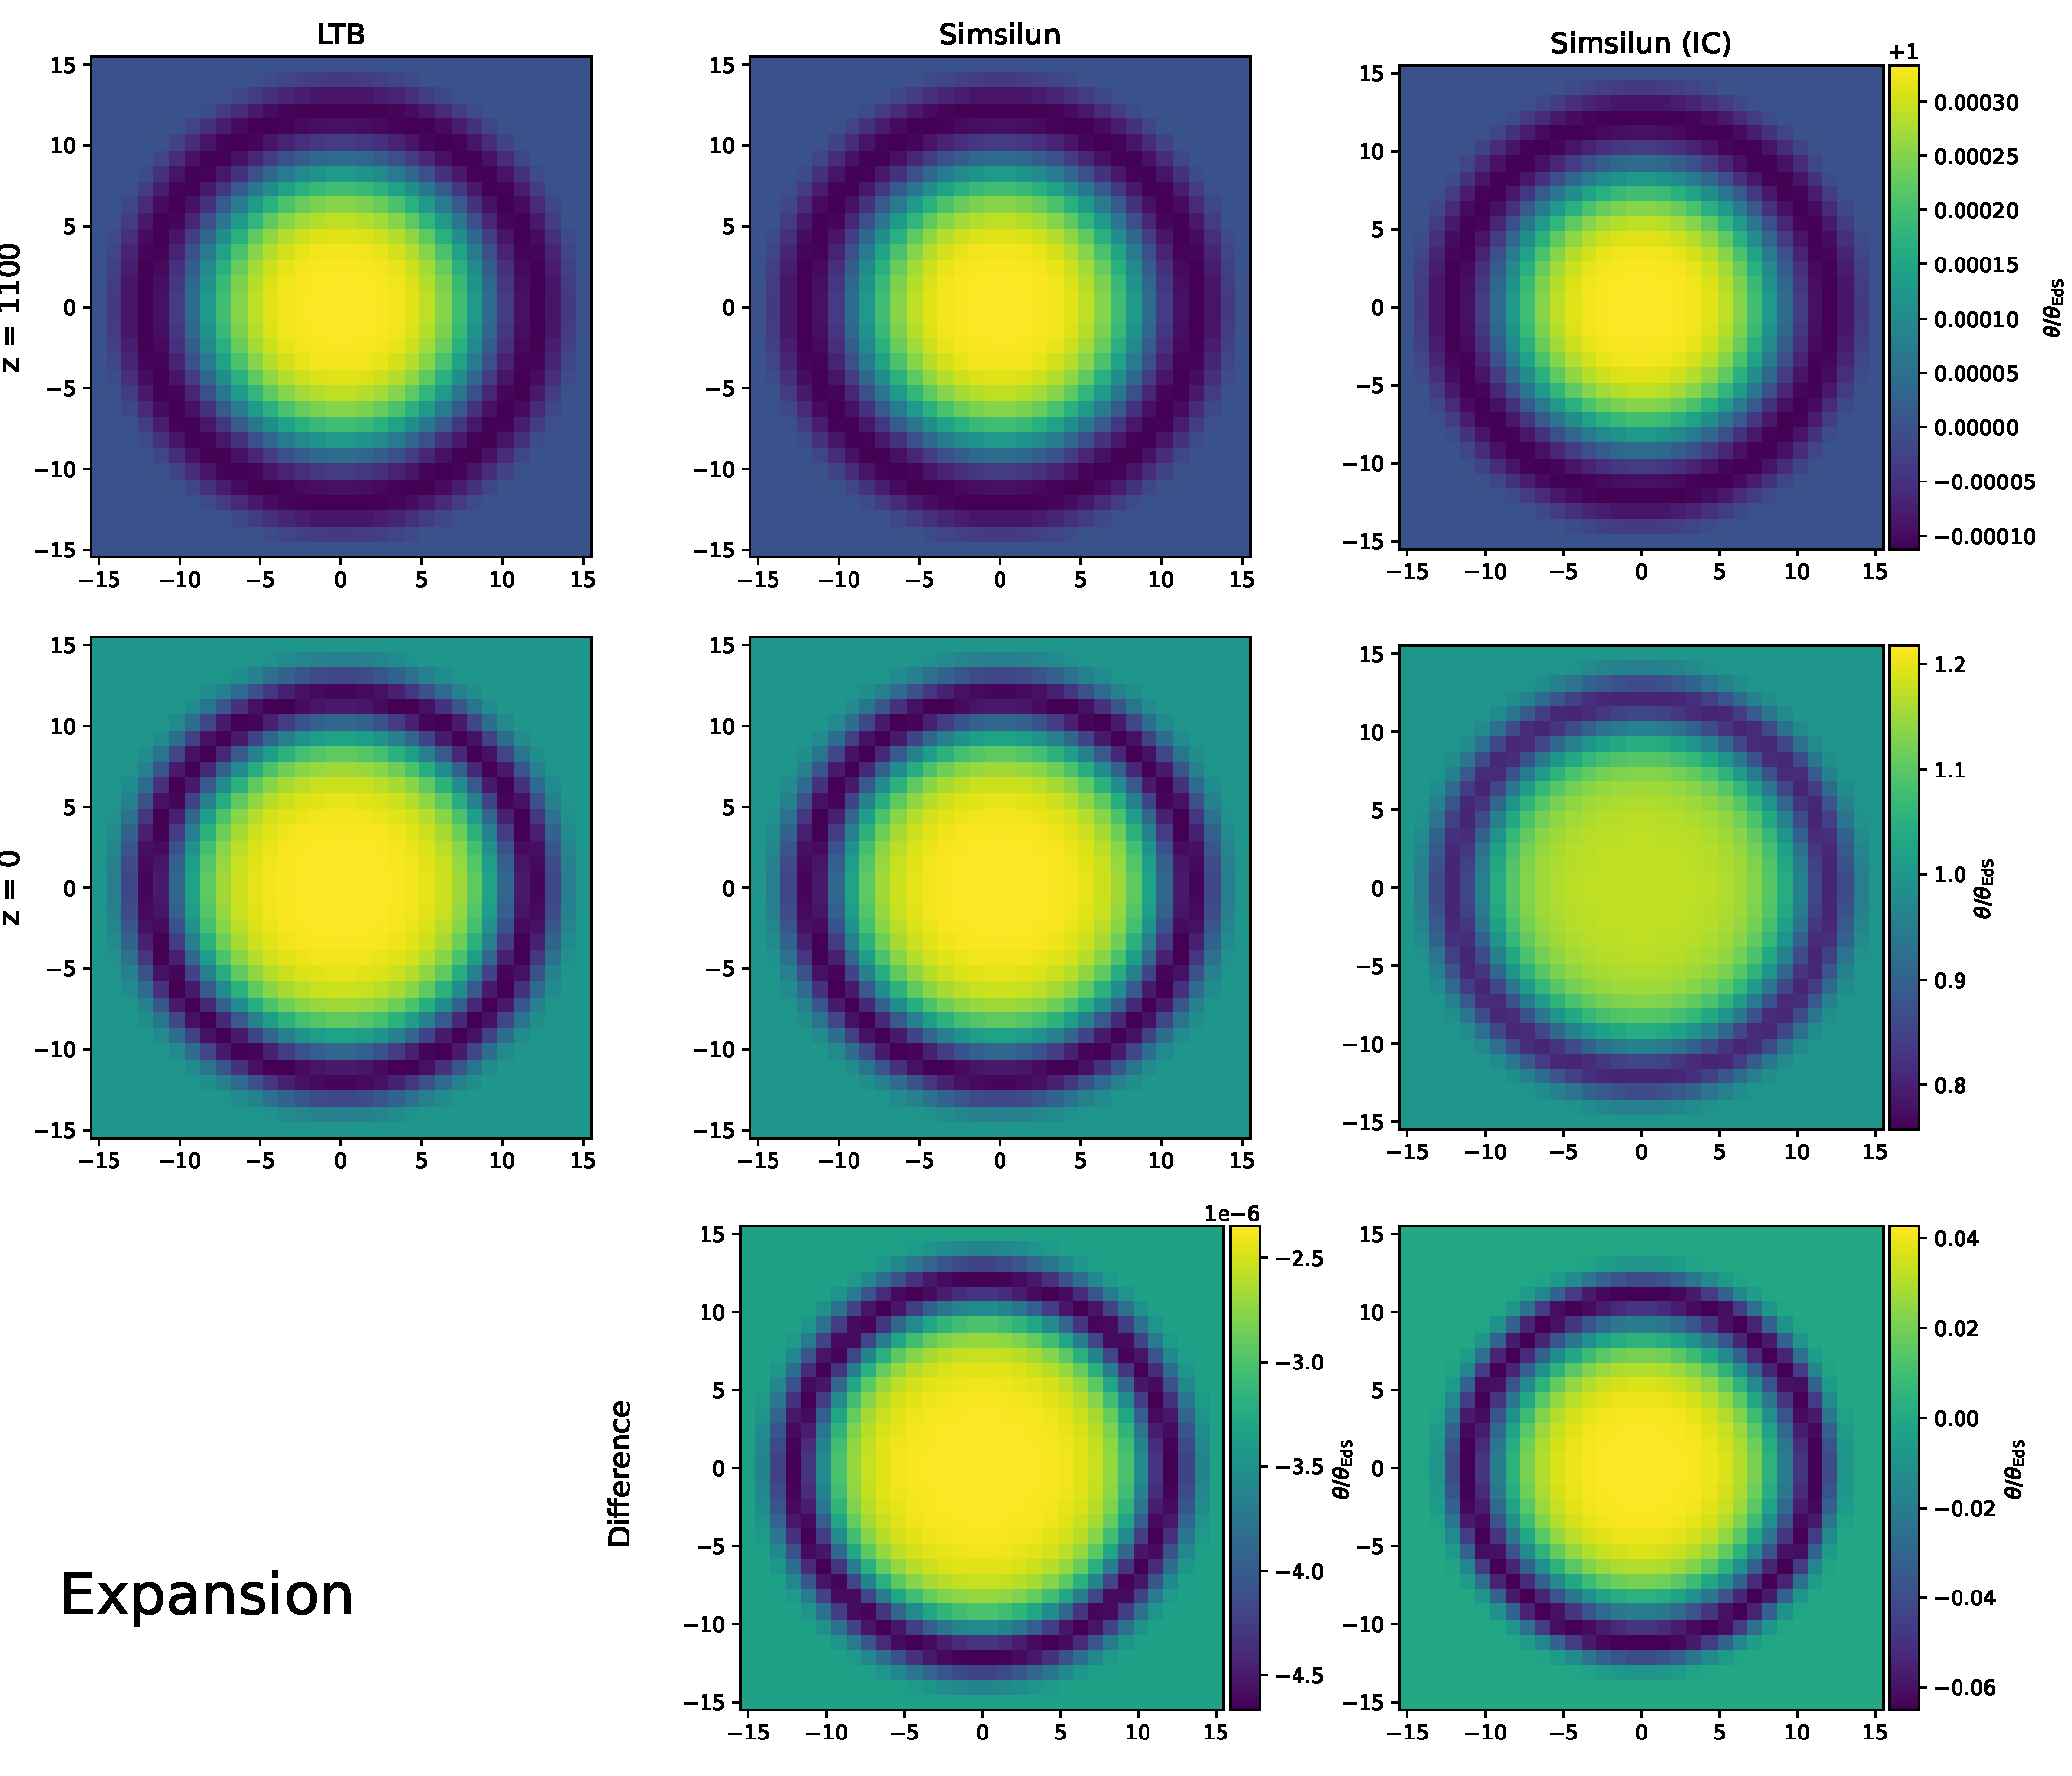
\includegraphics[width=\textwidth]{../plots/Expansion.pdf}
    \caption{Expansion}
    \label{fig:expansion}
\end{figure}



\begin{figure}
    \centering
    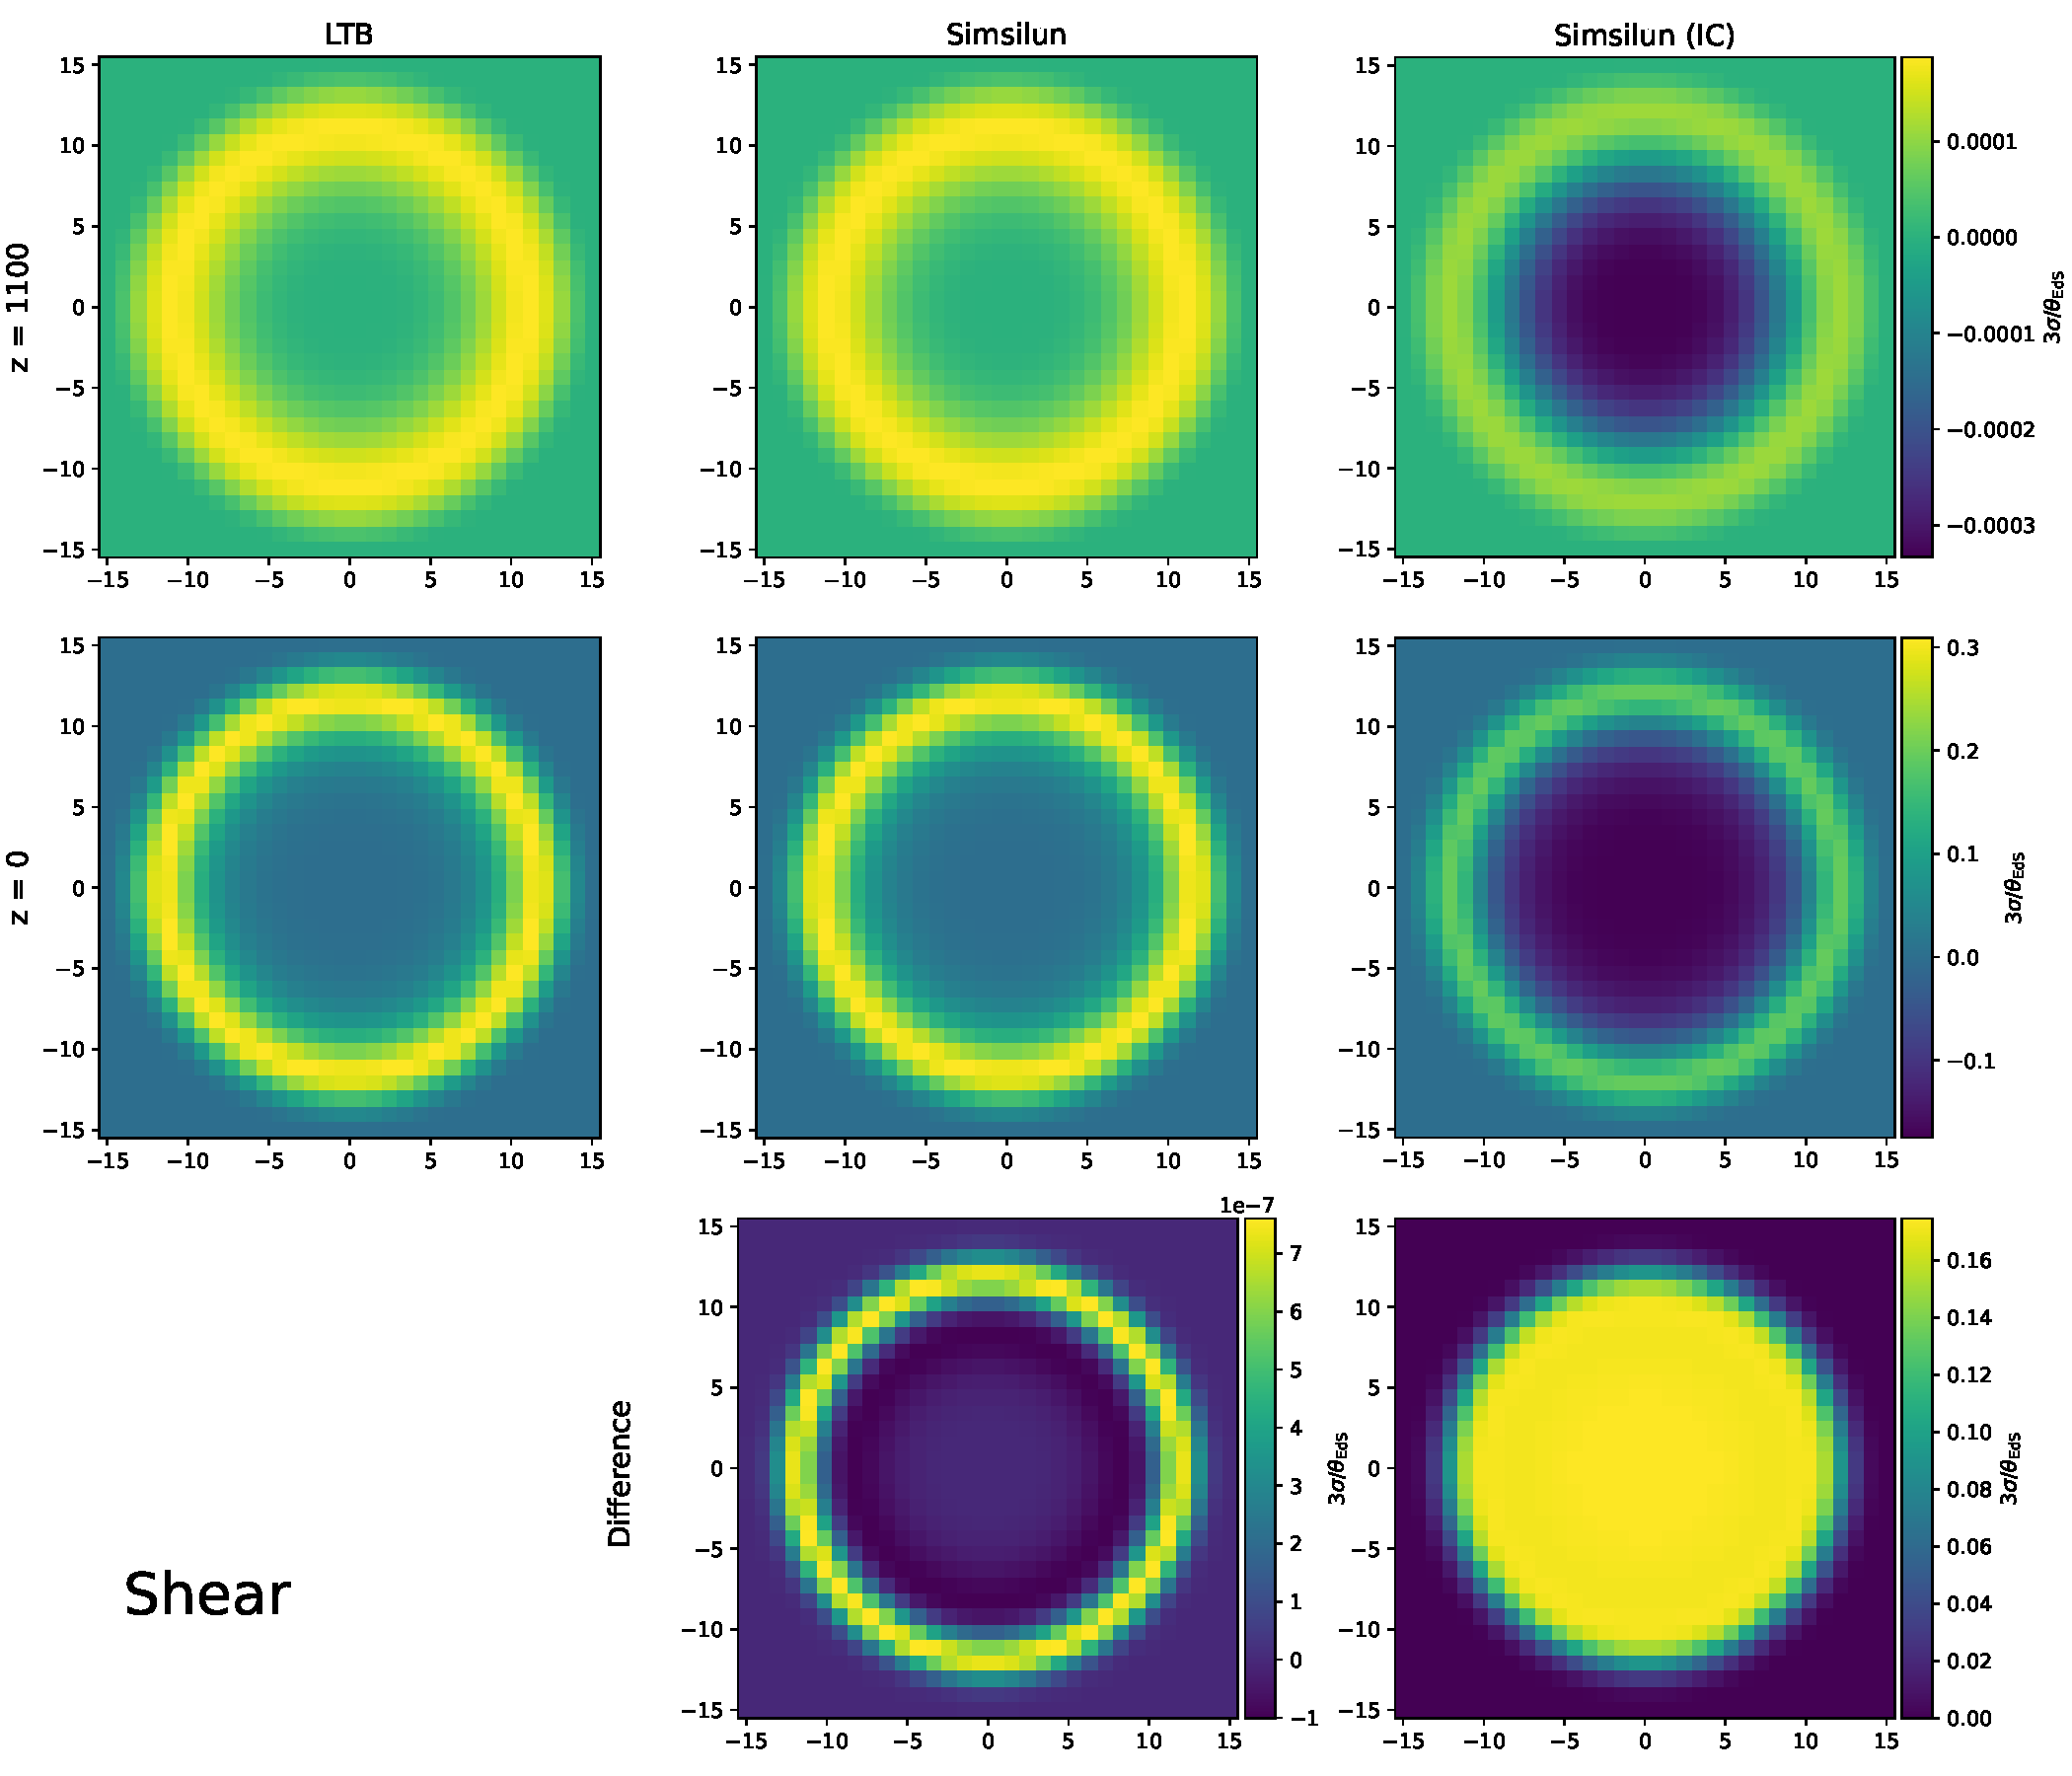
\includegraphics[width=\textwidth]{../plots/Shear.pdf}
    \caption{Shear}
    \label{fig:shear}
\end{figure}



\begin{figure}
    \centering
    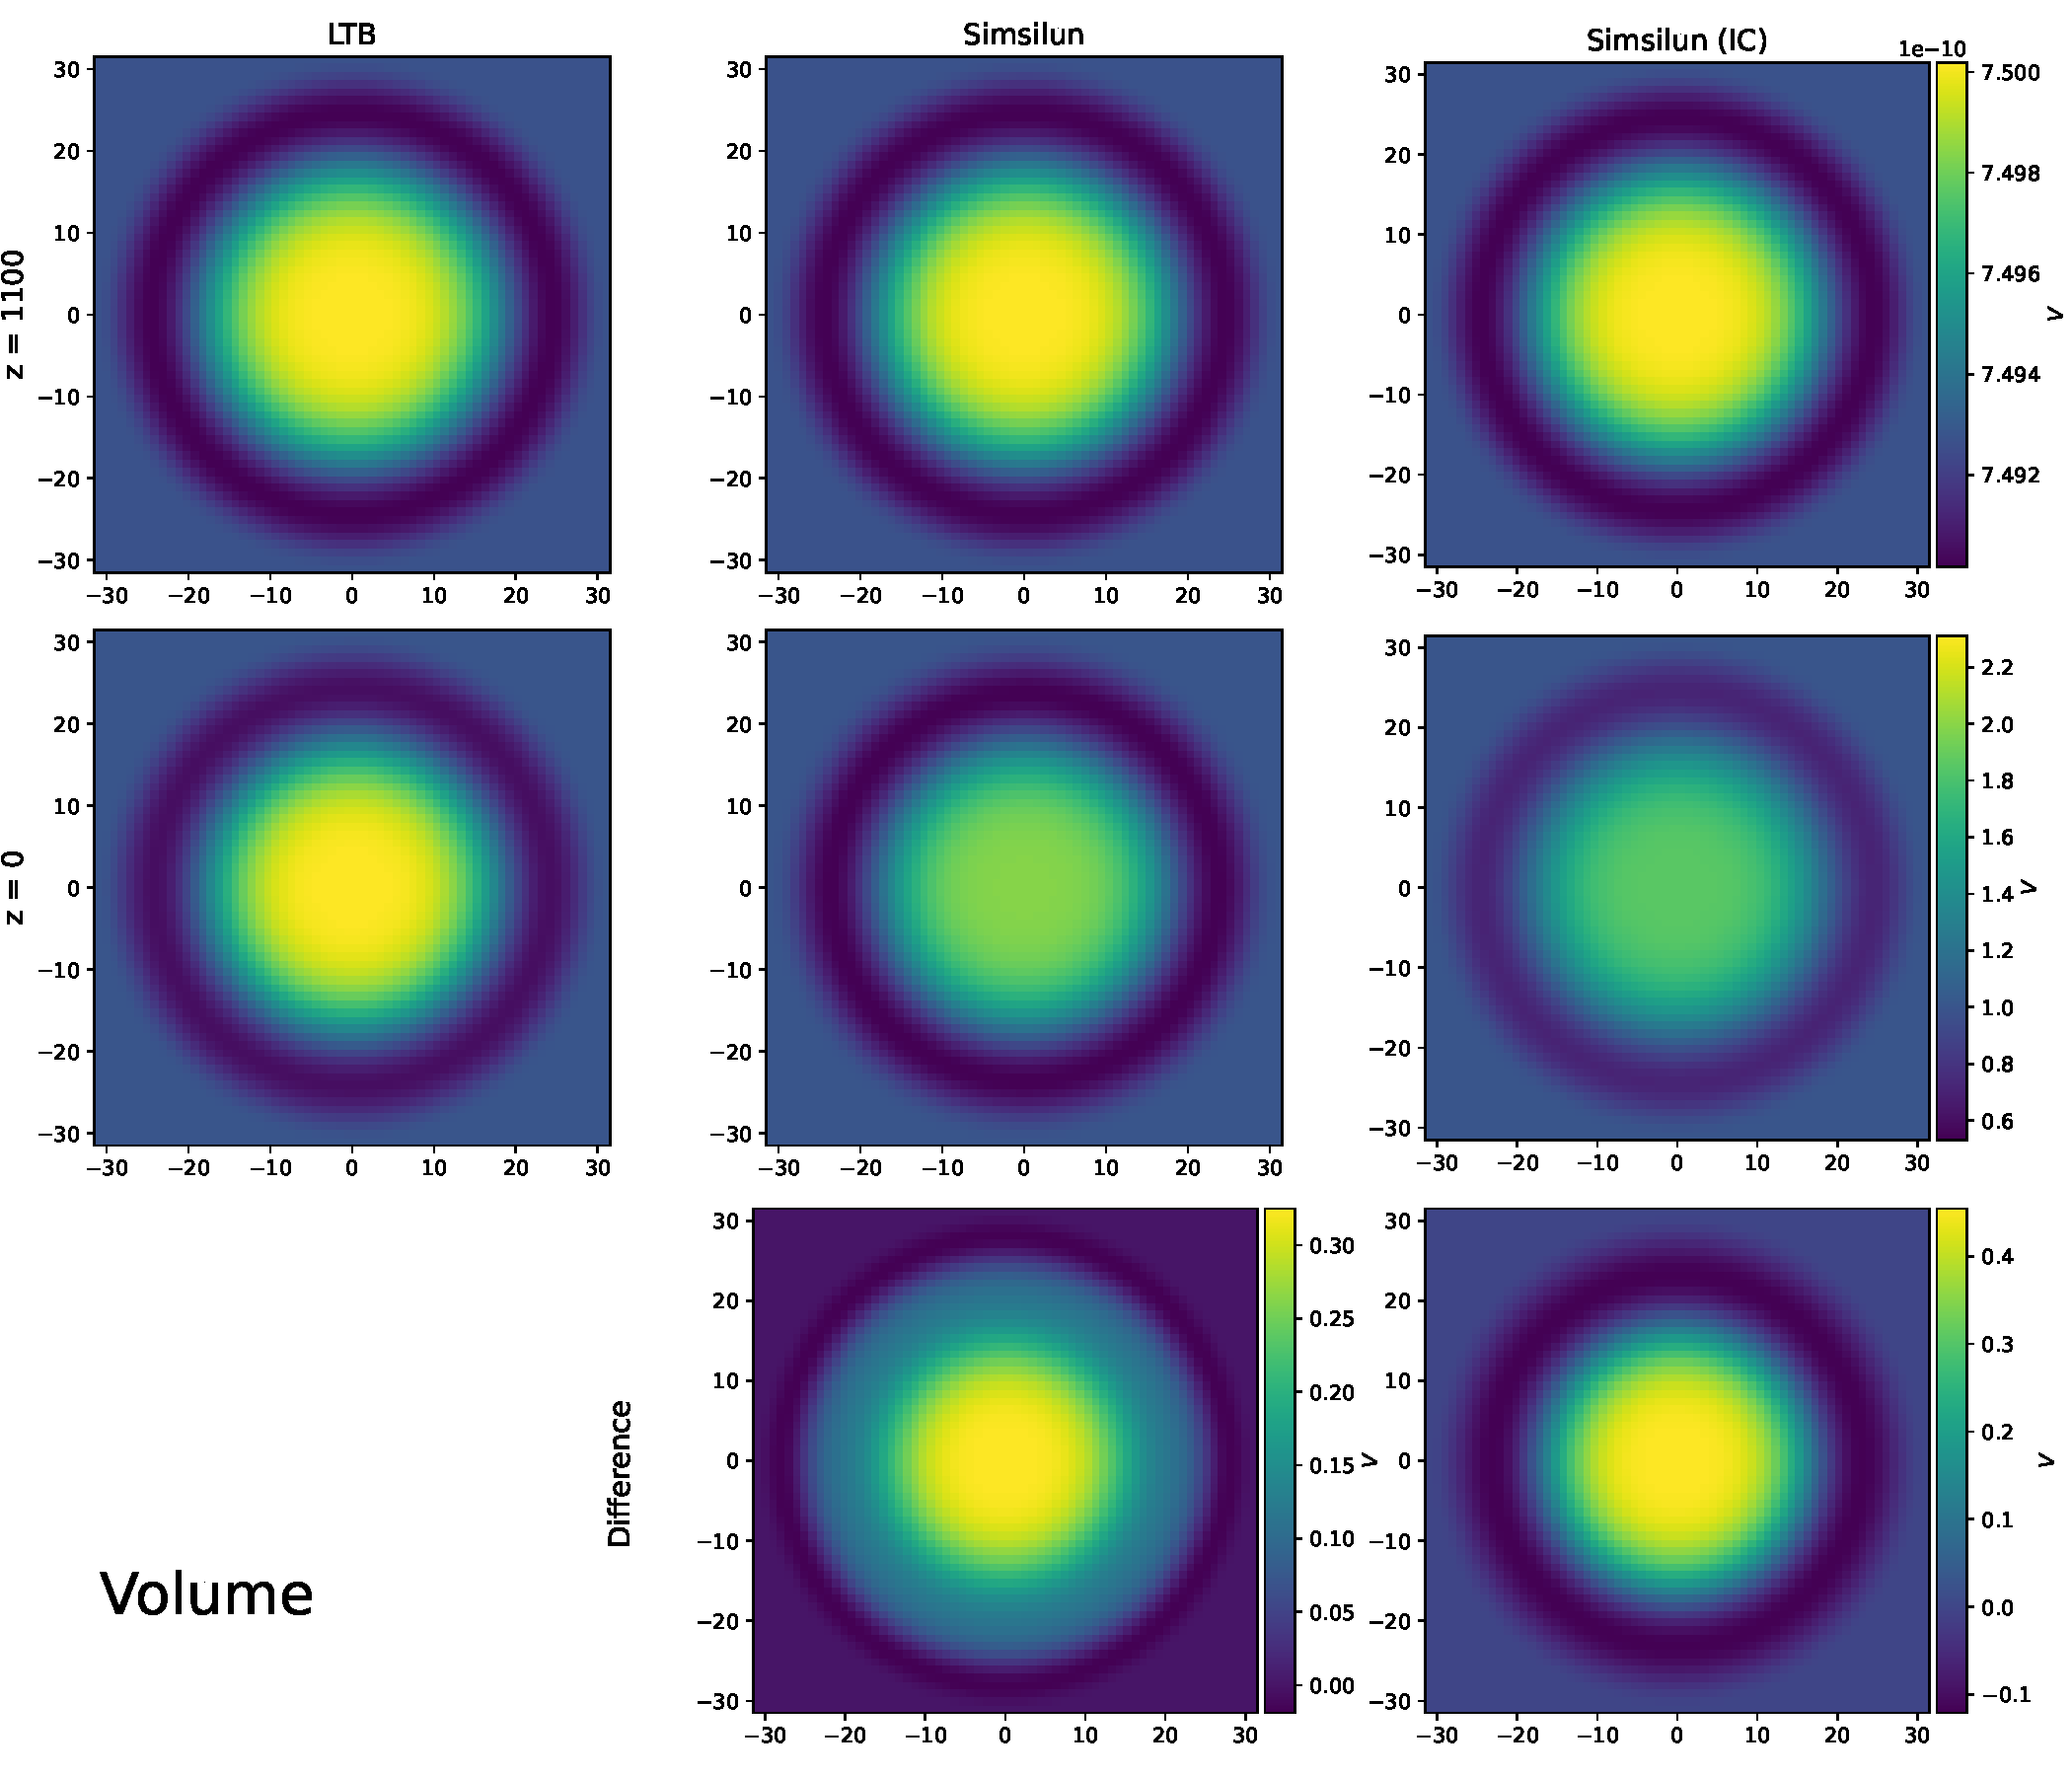
\includegraphics[width=\textwidth]{../plots/Volume.pdf}
    \caption{Volume}
    \label{fig:volume}
\end{figure}



\begin{figure}
    \centering
    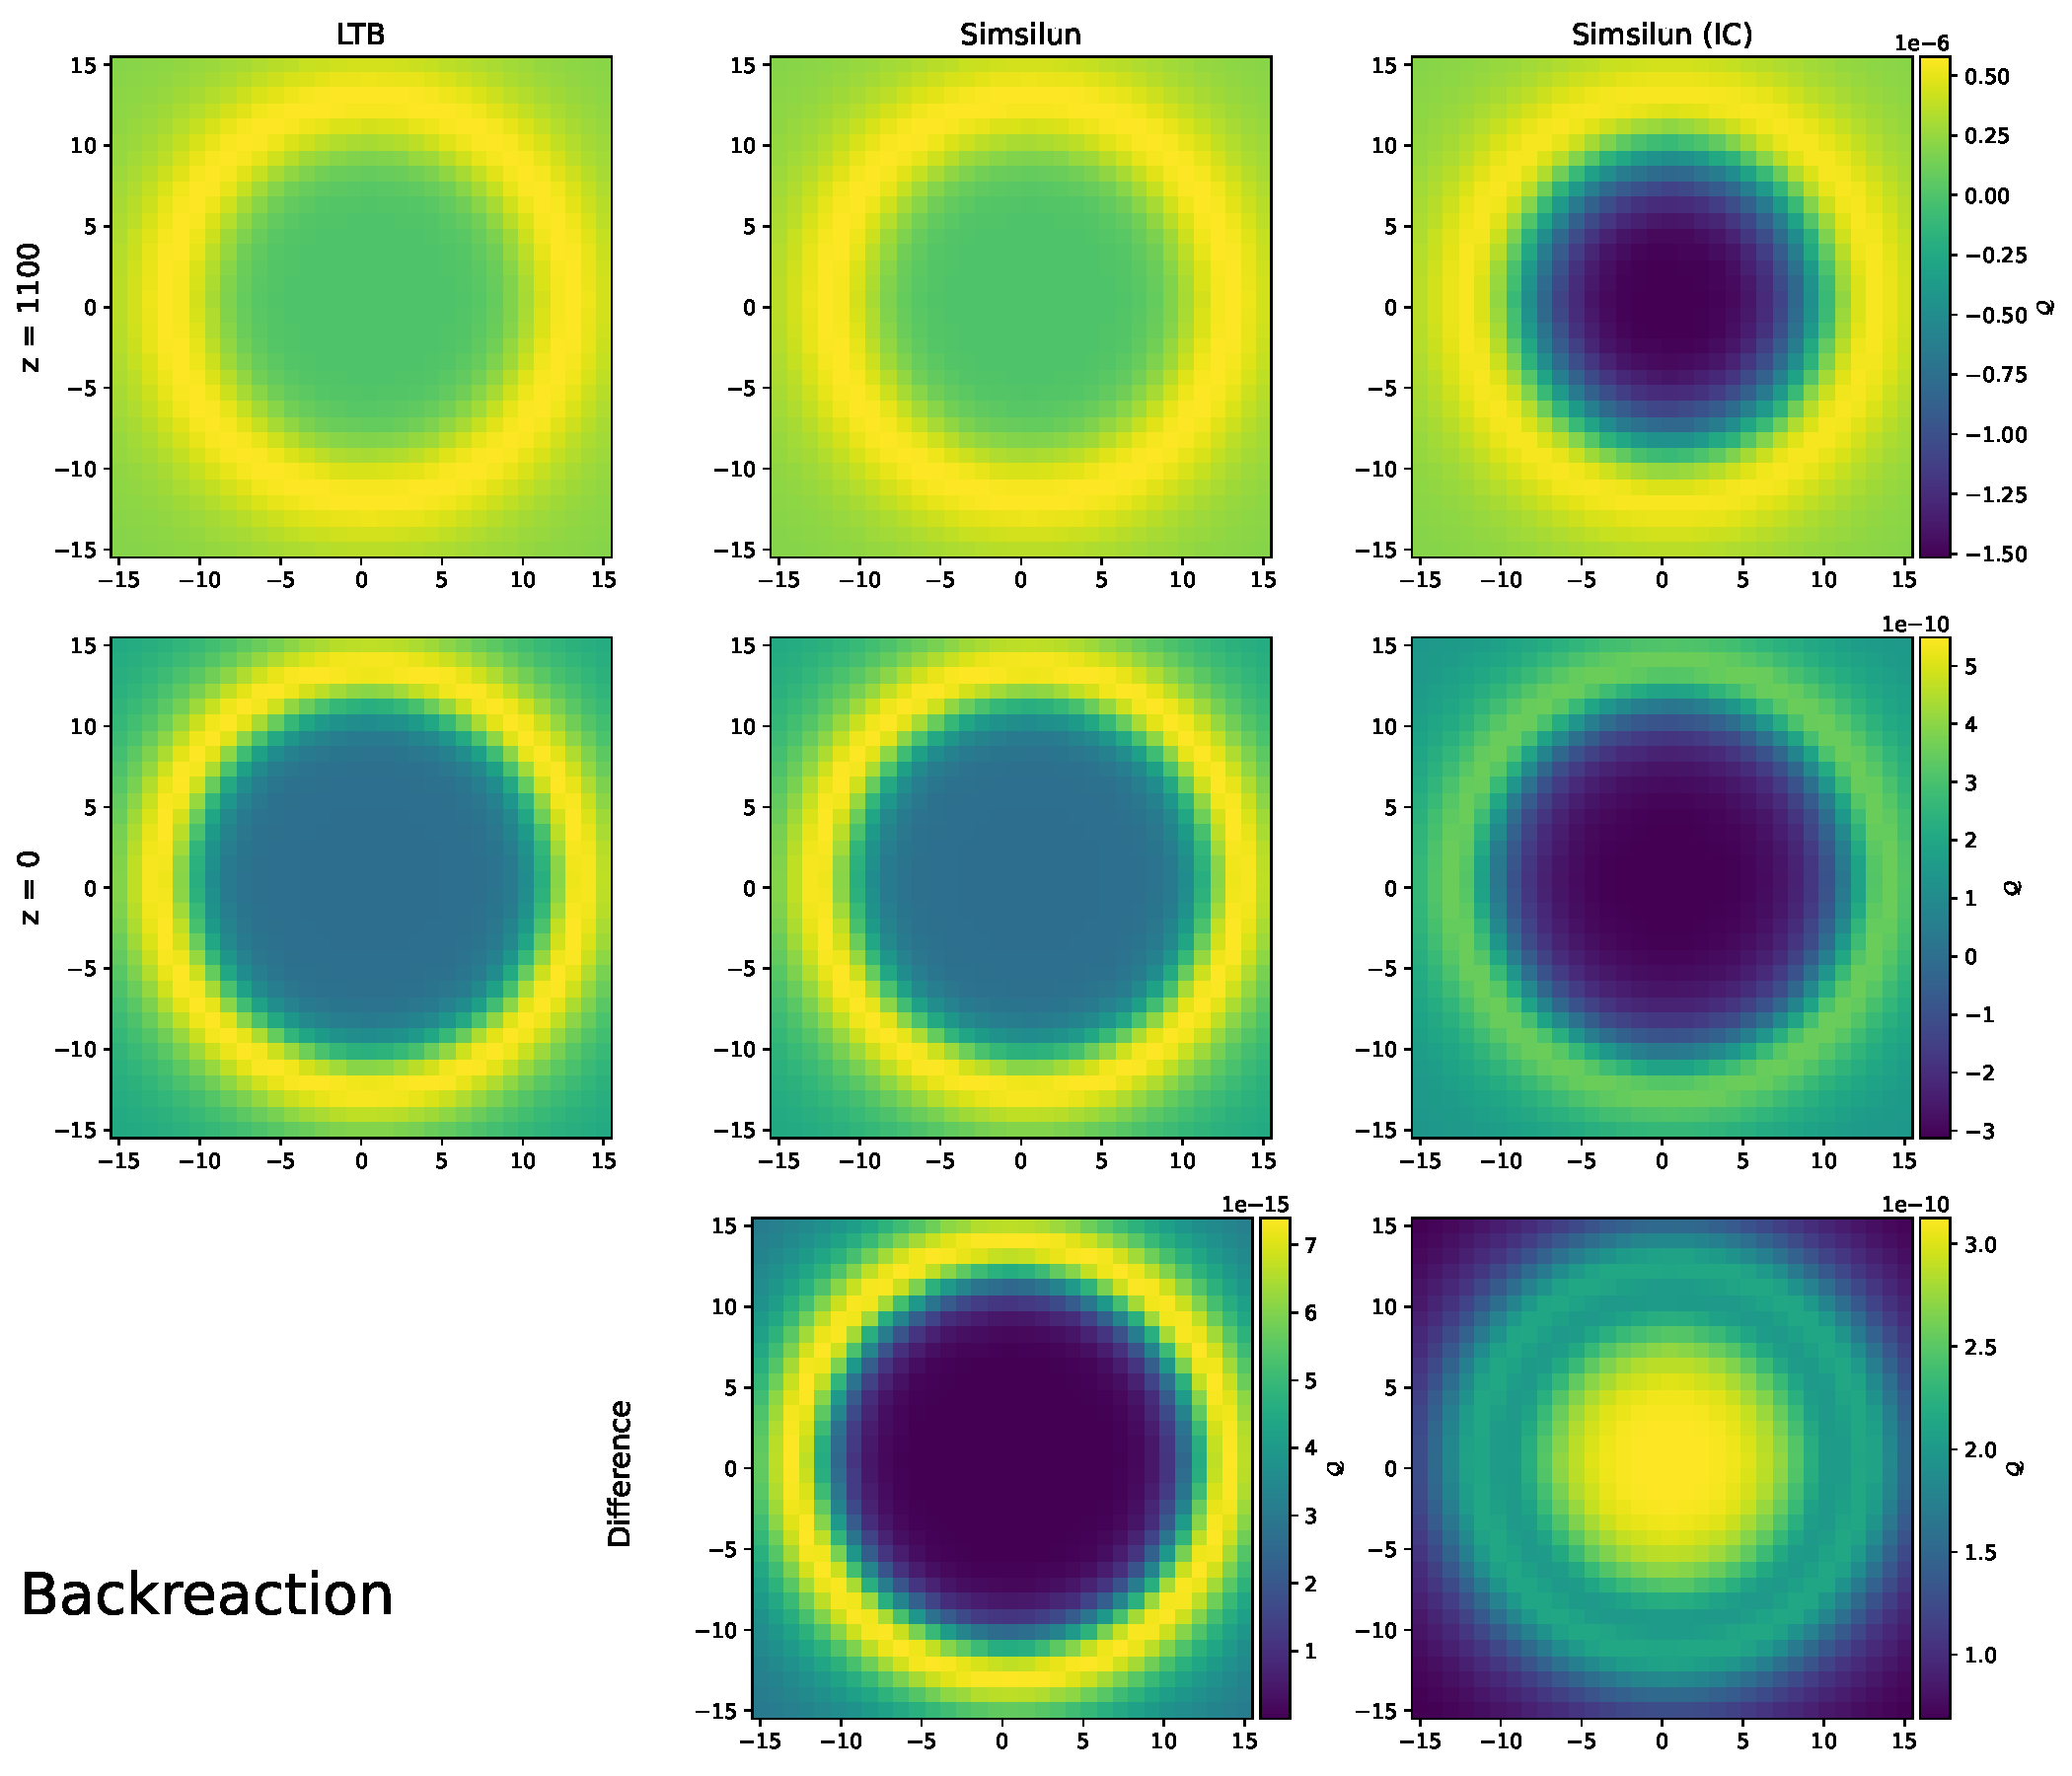
\includegraphics[width=\textwidth]{../plots/Backreaction.pdf}
    \caption{Backreaction}
    \label{fig:backreaction}
\end{figure}
\end{document}
